\documentclass[12pt]{article}
\usepackage[danish]{babel}
\usepackage{amsfonts, amssymb, mathtools, amsthm, amsmath}
\usepackage{graphicx, pgfplots}
\usepackage{url}
\usepackage[dvipsnames]{xcolor}
\usepackage{sagetex}
\usepackage{lastpage}

%loaded last
\usepackage[hidelinks]{hyperref}

\usepackage{siunitx}
  \sisetup{exponent-product = \cdot,
    output-decimal-marker = {,}}

%Giles Castelles incfig
\usepackage{import}
\usepackage{xifthen}
\usepackage{pdfpages}
\usepackage{transparent}

\newcommand{\incfig}[2][1]{%
  \def\svgwidth{#1\columnwidth}
  \import{../figures/}{#2.pdf_tex}
}

\setlength{\parindent}{0in}
\setlength{\oddsidemargin}{0in}
\setlength{\textwidth}{6.5in}
\setlength{\textheight}{8.8in}
\setlength{\topmargin}{0in}
\setlength{\headheight}{18pt}

\usepackage{fancyhdr}
\pagestyle{fancy}

\fancyhead{}
\fancyfoot{}
\fancyfoot[R]{\thepage}
\fancyhead[C]{\leftmark}

\pgfplotsset{compat=newest}

\pgfplotsset{every axis/.append style={
  axis x line=middle,    % put the x axis in the middle
  axis y line=middle,    % put the y axis in the middle
  axis line style={<->,color=black}, % arrows on the axis
}}

\usepackage{thmtools}
\usepackage{tcolorbox}
  \tcbuselibrary{skins, breakable}
  \tcbset{
    space to upper=1em,
    space to lower=1em,
  }

\theoremstyle{definition}

\newtcolorbox[auto counter]{definition}[1][]{%
  breakable,
  colframe=ForestGreen,  %frame color
  colback=ForestGreen!5, %background color
  colbacktitle=ForestGreen!25, %background color for title
  coltitle=ForestGreen!70!black,  %title color
  fonttitle=\bfseries\sffamily, %title font
  left=1em,              %space on left side in box,
  enhanced,              %more options
  frame hidden,          %hide frame
  borderline west={2pt}{0pt}{ForestGreen},  %display left line
  title=Definition \thetcbcounter: #1,
}

\newtcolorbox{greenline}{%
  breakable,
  colframe=ForestGreen,  %frame color
  colback=white,          %remove background color
  left=1em,              %space on left side in box
  enhanced,              %more options
  frame hidden,          %hide frame
  borderline west={2pt}{0pt}{ForestGreen},  %display left line
}

\newtcolorbox[auto counter, number within=section]{eks}[1][]{%
  brekable,
  colframe=NavyBlue,  %frame color
  colback=NavyBlue!5, %background color
  colbacktitle=NavyBlue!25,    %background color for title
  coltitle=NavyBlue!70!black,  %title color
  fonttitle=\bfseries\sffamily, %title font
  left=1em,            %space on left side in box,
  enhanced,            %more options
  frame hidden,        %hide frame
  borderline west={2pt}{0pt}{NavyBlue},  %display left line
  title=Eksempel \thetcbcounter: #1
}

\newtcolorbox{blueline}{%
  breakable,
  colframe=NavyBlue,     %frame color
  colback=white,         %remove background
  left=1em,              %space on left side in box,
  enhanced,              %more options
  frame hidden,          %hide frame
  borderline west={2pt}{0pt}{NavyBlue},  %display left line
}

\newtcolorbox{teo}[1][]{%
  breakable,
  colframe=RawSienna,  %frame color
  colback=RawSienna!5, %background color
  colbacktitle=RawSienna!25,    %background color for title
  coltitle=RawSienna!70!black,  %title color
  fonttitle=\bfseries\sffamily, %title font
  left=1em,              %space on left side in box,
  enhanced,              %more options
  frame hidden,          %hide frame
  borderline west={2pt}{0pt}{RawSienna},  %display left line
  title=Teori: #1,
}

\newtcolorbox[auto counter, number within=section]{sæt}[1][]{%
  breakable,
  colframe=RawSienna,  %frame color
  colback=RawSienna!5, %background color
  colbacktitle=RawSienna!25,    %background color for title
  coltitle=RawSienna!70!black,  %title color
  fonttitle=\bfseries\sffamily, %title font
  left=1em,              %space on left side in box,
  enhanced,              %more options
  frame hidden,          %hide frame
  borderline west={2pt}{0pt}{RawSienna},  %display left line
  title=Sætning \thetcbcounter: #1,
  before lower={\textbf{Bevis:}\par\vspace{0.5em}},
  colbacklower=RawSienna!25,
}

\newtcolorbox{redline}{%
  breakable,
  colframe=RawSienna,  %frame color
  colback=white,       %Remove background color
  left=1em,            %space on left side in box,
  enhanced,            %more options
  frame hidden,        %hide frame
  borderline west={2pt}{0pt}{RawSienna},  %display left line
}

\newtcolorbox{for}[1][]{%
  breakable,
  colframe=NavyBlue,  %frame color
  colback=NavyBlue!5, %background color
  colbacktitle=NavyBlue!25,    %background color for title
  coltitle=NavyBlue!70!black,  %title color
  fonttitle=\bfseries\sffamily, %title font
  left=1em,              %space on left side in box,
  enhanced,              %more options
  frame hidden,          %hide frame
  borderline west={2pt}{0pt}{NavyBlue},  %display left line
  title=Forklaring #1,
}

\newtcolorbox{bem}{%
  breakable,
  colframe=NavyBlue,  %frame color
  colback=NavyBlue!5, %background color
  colbacktitle=NavyBlue!25,    %background color for title
  coltitle=NavyBlue!70!black,  %title color
  fonttitle=\bfseries\sffamily, %title font
  left=1em,              %space on left side in box,
  enhanced,              %more options
  frame hidden,          %hide frame
  borderline west={2pt}{0pt}{NavyBlue},  %display left line
  title=Bemærkning:,
}

\makeatother
\def\@lecture{}%
\newcommand{\lecture}[3]{
  \ifthenelse{\isempty{#3}}{%
    \def\@lecture{Lecture #1}%
  }{%
    \def\@lecture{Lecture #1: #3}%
  }%
  \subsection*{\makebox[\textwidth][l]{\@lecture \hfill \normalfont\small\textsf{#2}}}
}

\makeatletter

\newcommand{\opgave}[1]{%
 \def\@opgave{#1}%
 \subsection*{Opgave #1}
}

\makeatother

%Format lim the same way in intext and in display
\let\svlim\lim\def\lim{\svlim\limits}

% horizontal rule
\newcommand\hr{
\noindent\rule[0.5ex]{\linewidth}{0.5pt}
}

\title{Opgaver til forelæsning 20}
\author{Noah Rahbek Bigum Hansen}
\date{20. November 2024}

\begin{document}

\maketitle

\section*{Opg. 13.31}
The star $\mathrm{Rho}^1$ Cancri is 57 light-years from the earth and has a mass \num{0,85} times that of our sun. A planet has been detected in a circular orbit around $\mathrm{Rho}^1$ with an orbital radius equal to \num{0,11} times the radius of the earth's orbit around the sun. What are

\subsection*{(a)}
The orbital speed of the planet of Rho$^1$ Cancri?
\bigbreak
Vi har formlen for hastigheden, $v$, i en jævn tyngdebundet cirkelbevægelse som
\[ 
v = \sqrt{\frac{GM}{r}} = \sqrt{\frac{G\cdot \num{0,85} \cdot \qty{1,99e30}{kg}}{\num{0,11} \cdot \qty{1,5e8}{km}}} = \qty{82720}{\frac{m}{s}} 
.\]


\subsection*{(b)}
The orbital period of the planet of $\mathrm{Rho}^1$ Cancri?
\bigbreak
Formlen for perioden for et objekt i en tyngdebundet jævn cirkelbevægelse er
\[ 
T = \frac{2\pi r^{\frac{3}{2}}}{\sqrt{GM}} = \frac{2\pi (\num{0,11} \cdot \qty{1,5e8}{km})^{\frac{3}{2}}}{\sqrt{G \cdot \num{0,85} \cdot \qty{1,99e30}{kg}}} = \qty{1,254e6}{s} \cong \qty{14,5}{days}
.\]


\section*{Opg. 13.35}
A thin spherical shell has radius $r_A = \qty{4,00}{m}$ and mass
$m_A = \qty{20,0}{kg}$. It is concentric with a second thin spherical shell that has radius $r_B = \qty{6,00}{m}$ and mass $m_B = \qty{40,0}{kg}$. What is the net gravitational force that the two shells exert on a point mass of \qty{0,0200}{kg}  that is a distance $r$ from the common center of the two shells.

\subsection*{(a)}
$r = \qty{2,00}{m}$ (inside both shells)
\bigbreak
Fra Newtons skalteorem har vi at tyngdefeltet indeni en hul skal er 0. I dette tilfælde er massen placeret indeni begge skaller og derfor er det effektive tyngdefelt 0.

\subsection*{(b)}
$r = \qty{5,00}{m}$ (in the space between the two shells
\bigbreak
Her er det kun den inderste masse der bidrager til tyngdefeltet. Vi får
\[ 
F_g = \frac{GMm}{r^2} = \frac{G\cdot \qty{20,0}{kg} \cdot \qty{0,0200}{kg}}{(\qty{5,00}{m} )^2} = \qty{1,07e-12}{N}  
.\]


\subsection*{(c)}
$r = \qty{8,00}{m}$ (outside both shells)
\bigbreak
Her bidrager den yderste skal også så vi får
\[ 
F_g = \frac{Gm}{r^2}(m_a + m_b) = \frac{G \cdot \qty{0,0200}{kg}}{(\qty{8,00}{m})^2}(\qty{20,0}{kg} + \qty{40,0}{kg}) = \qty{1,25e-12}{N} 
.\]


\section*{Opg. 13.37}
A uniform, solid, \qty{1000,0}{kg} sphere has a radius of \qty{5,00}{m}.

\subsection*{(a)}
Find the gravitational force the sphere exerts on a \qty{2,00}{kg} point mass placed at the following distances from the center of the sphere

\subsubsection*{(i)}
\qty{5,01}{m} 
\bigbreak
Vi benytter gravitationsloven som
\[ 
F_g = \frac{GMm}{r^2} = \qty{5,34e-9}{N} 
.\]


\subsubsection*{(ii)}
\qty{2,50}{m} 
\bigbreak
Fra Eksempel 13.10 har vi gravitationskraften, $F_g$, som
\[ 
F_g = \frac{GMm}{R^3}r
,\]
hvor $R$ er radius af objektet og $r$ er afstanden til objektets centrum. Vi har altså
\[ 
F_g = \frac{G \cdot \qty{1000,0}{kg} \cdot \qty{2,00}{kg} }{(\qty{5,00}{m})^3} \cdot \qty{2,50}{m} = \qty{2,67e-9}{N}  
.\]


\subsection*{(b)}
Sketch a qualitative graph of the magnitude of the gravitational force this sphere exerts on a point mass $m$ as a function of the distance $r$ of $m$ from the center of the sphere. Include the region from $r = 0$ to $r \to \infty$.
\bigbreak
\begin{figure}[ht]
  \centering
  \incfig[0.8]{F19_13_37}
  \caption{Tegning af situationen}
  \label{fig:F19_13_37}
\end{figure}
Se \textbf{\autoref{fig:F19_13_37}}

\section*{Opg. 13.39}
\begin{figure} [ht]
  \centering
  \caption{}
  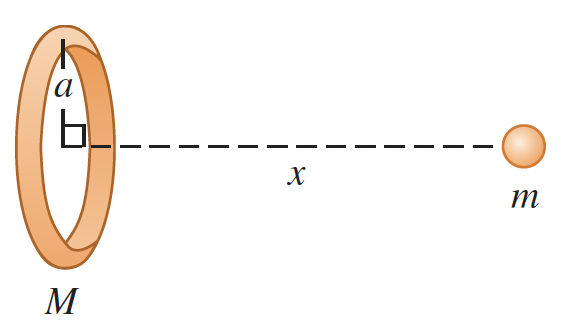
\includegraphics[width=0.6\linewidth]{../figures/E13_39.png}
  \label{fig:E13_39}
\end{figure}

Consider the ringshaped object in \textbf{\autoref{fig:E13_39}}. A particle with mass $m$ is placed a distance $x$ from the center of the ring, along the line through the center of the ring and perpendicular to its plane.

\subsection*{(a)}
Calculate the gravitational potential energy $U$ of this system. Take the potential energy to be zero when the two objects are far apart.
\bigbreak
Afstanden fra $m$ til et punkt på cirkelperiferien $s = \sqrt{x^2 + a^2}$ er konstant for alle punkter på cirkelperiferien. Derudover sørger ringens symmetri for at enhver del af massen der ikke trækker parallelt i $m$ ift. $x$ har en masse netop modsat midten der trækker ligeså meget i den anden retning og derfor er den potentielle gravitationelle energi
\[ 
U_g = - \frac{GMm}{\sqrt{x^2 + a^2}}
.\]

\subsection*{(b)}
Show that your answer to part (a) reduces to the expected result when $x$ is much larger than the radius a of the ring.
\bigbreak
For $x \to \infty$ er $a \ll x$ og derfor fås at
\[ 
\lim_{x \to \infty } U_g = -\frac{GMm}{x}
.\]



\subsection*{(c)}
Use $F_x = - \frac{\mathrm{d}U}{\mathrm{d}x}$ to find the magnitude and direction of the force on the particle (see Section 7.4).
\bigbreak
Vi løser so så.
\[ 
F_x = - \frac{\mathrm{d}U}{\mathrm{d}x} = \frac{\mathrm{d}}{\mathrm{d}x} \frac{GMm}{\sqrt{x^2 + a^2}} = - \frac{GMmx}{\left( x^2 + a^2 \right)^{\frac{3}{2}}}
.\]


\subsection*{(d)}
Show that your answer to part (c) reduces to the expected result when $x$ is much larger than $a$.
\bigbreak
\[ 
\lim_{x \to \infty} F_x = - \frac{GMmx}{x^3} = - \frac{GMm}{x^2}
.\]


\subsection*{(e)}
What are the values of $U$ and $F_x$ when $x = 0$? Explain why these results make sense.
\bigbreak
For $x = 0$ har vi
\begin{align*}
  U_g &= - \frac{GMm}{a} \\
  F_x &= 0
.\end{align*}


\section*{Opg. 13.71}
Planets are not uniform inside. Normally, they are densest at the center and have decreasing density outward toward the surface. Model a spherically symmetric planet, with the same radius as the earth, as having a density that decreases linearly with distance from the center. Let the density be \qty{15,0e3}{kg/m^3}  at the center and \qty{2,0e3}{kg/m^3}  at the surface. What is the acceleration due to gravity at the surface of this planet?
\bigbreak
Vi kan opstille følgende funktion for densiteten af planeten som funktion af afstanden til centrum $r$. 
\[ 
\rho(r) = (\rho_R - \rho_0)\frac{r}{R} + \rho_0
.\]
Den gravitationelle acceleration ved overfladen kun af planetens radius og af dens masse. Planetens radius er kendt og derfor skal kun dens masse findes. Dette gøres ved at inddele planeten i en række tynde skaller, der hver har volumenet
\[ 
\mathrm{d}V = 4\pi r^2 \, \mathrm{d}r
.\]
Vi får altså
\begin{align*}
  M &= \int_{0}^{R_E} 4\pi r^2 \rho(r) \, \mathrm{d}r \\
    &= 4\pi \left( \rho_0 \int_{0}^{R_E} r^2 \, \mathrm{d}r - \frac{\rho_0 - \rho_R}{R} \int_{0}^{R_E} r^3 \, \mathrm{d}r \right)  \\
    &= 4\pi \left( \rho_0 \frac{R^3}{3} - \frac{\rho_0 - \rho_R}{R} \frac{R^{4}}{4} \right) \\
    &= 4\pi R^3 \left( \frac{\rho_0}{3} - \frac{\rho_0 - \rho_R}{4} \right) \\
    &= \pi R^3 \left( \rho_R + \frac{1}{3}\rho_0 \right)
.\end{align*}

Vi kan dermed benytte formlen for tyngdeacceleration ved overfladen af en planet
\[ 
g = \frac{GM}{R^2} = GR\pi \left( \rho_R + \frac{1}{3}\rho_0 \right) = \pi G \cdot \qty{6378}{km} \left( \qty{2,0e3}{\frac{kg}{m^3}} + \frac{1}{3} \cdot \qty{15,0e3}{\frac{kg}{m^3}}  \right) =  \qty{9,361}{\frac{m}{s^2}} 
.\]


\section*{Opg. 13.73}
An object in the shape of a thin ring has radius $a$ and mass $M$. A uniform sphere with mass $m$ and radius $R$ is placed with its center at a distance $x$ to the right of the center of the ring, along a line through the center of the ring, and perpendicular to its plane (see \autoref{fig:E13_39}). What is the gravitational force that the sphere exerts on the ring-shaped object? Show that your result reduces to the expected result when $x$ is much larger than $a$.
\bigbreak
Se Opg. 13.39

\end{document}
